\section{Hyper parameter tuning}\label{ch:hyper_parameter_tuning}

Unfortunately there is no obvious optimal model for each problem.
A model maps input to output.
To reliably determine which information is to be discarded (and thus does not help to generalize) and which to emphasize, assumptions have to be made. % TODO terrible sentence

In 1996 David Wolpert pointed out that if no assumptions are made on the dataset there is no reason to prefer one model over another.
This line of reasoning is now known as the \textit{No Free Lunch Theorem} \cite{Wolpert1996}.
Some of these assumptions are already made beforehand (e.g. the usage of feed forward neural networks), but others are subject to optimization. % TODO terrible sentence

Hyper-parameter optimization is an optimization problem by minimizing the loss (or another metric like accuracy) of the model on the given training data.
Hyper parameters used in the first model which may be object to optimize are:

\begin{enumerate}
    \item Training data:
    \begin{tasks}(2)
        \task Number of training examples
        \task Image size
        \task Batch size
        \task Feature reduction
    \end{tasks}
    \item Model:
    \begin{tasks}(2)
        \task Number of layers
        \task Layer type
        \task Layer size
        \task Loss function
    \end{tasks}
    \item Optimizer:
    \begin{tasks}(2)
        \task Type of optimizer
        \task Learning rate
        \task Momentum
        \task Nesterov
    \end{tasks}
    \item Training:
    \begin{tasks}(2)
        \task Steps per epoch
        \task Number of epochs
    \end{tasks}
\end{enumerate}

Some hyper-parameters have to be tested and are not obvious, but others can be improved without any obvious negative side effects so they are discussed first. Then algorithms to test different models with different hyper-parameters to improve the model are explored.

\subsection{Data augmentation}\label{ch:data_augmentation}
% TODO Add citation to Chollet p.138
% TODO Add dropout layer Chollet p.140
The first thing which can be improved is the size of the dataset we use to train the model.
In the previous tests the models saw every image approximately 20 times during training (batches of size 20, 20 steps per epoch and 20 epochs divided by 400 training samples), which is most likely the source of the occurring overfitting.
To increase the training set size thereby seems to be a reasonable approach.

Data augmentation on images changes some properties of the image which are reasonable for the purpose at hand.
In the case of symbol detection the symbol may be rotated or mirrored thus adding training examples without adding much redundancy to the dataset and in this very case not invalidating the data.

Data augmentation is performed by adjusting the \code{create\_generator} function used before:

\begin{lstlisting}
from tensorflow.keras.preprocessing.image import ImageDataGenerator

def create_generator(data_dir, batch_size, datagen):
    full_path = join(processed, data_dir)
    return datagen.flow_from_directory(
        full_path,
        target_size=(32, 32),
        batch_size=batch_size,
        class_mode='binary')

train_datagen = ImageDataGenerator(
        rescale = 1./255,
        rotation_range=360,
        horizontal_flip=True,
        vertical_flip=True)

test_datagen = ImageDataGenerator(rescale = 1./255)

train_generator = create_generator('train', 20, train_datagen)
test_generator = create_generator('test', 10, test_datagen)
\end{lstlisting}

Instead of \code{datagen = ImageDataGenerator(rescale = 1./255)} this object is given as parameter, because the training set adds random deviations to the loaded data.
Namely a random rotation and a chance to be horizontally and vertically flipped.
Please note that no deviations are applied to the test data.

Applying these changes gives a loss of 0.61 and a 78.75\% accuracy on the training data.
Loss and accuracy on the test set are 0.63 and 78\% respectively.

\begin{figure}
    \centering
    \begin{subfigure}[b]{0.4\textwidth}
        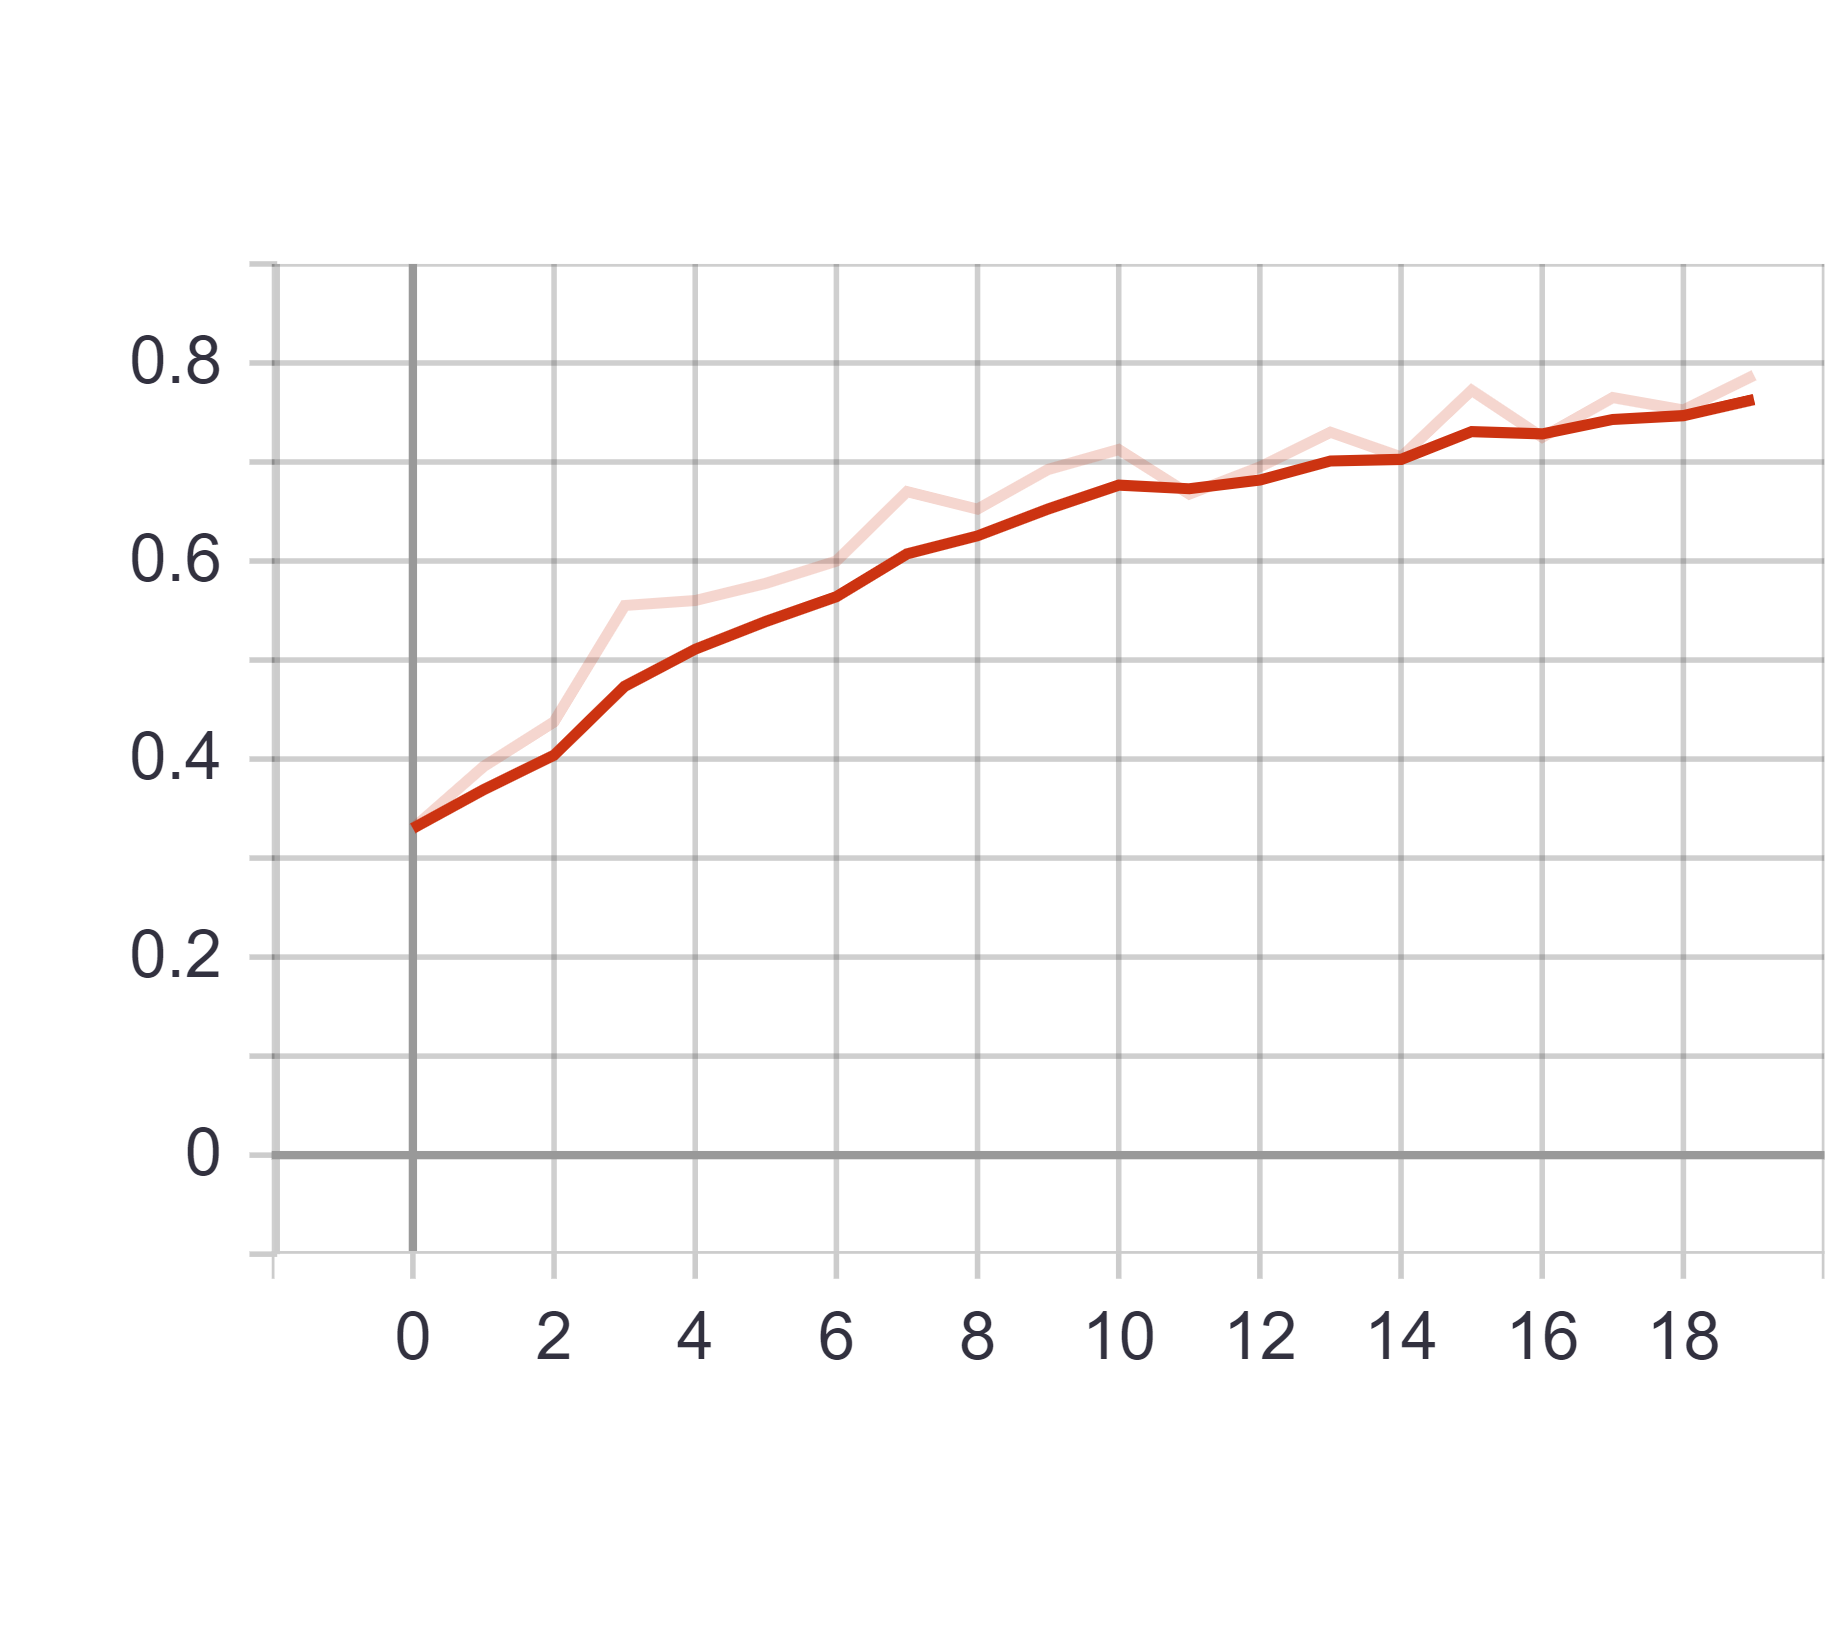
\includegraphics[width=\textwidth]{images/first_model_data_augmentation_acc.png}
        \caption{Accuracy}
        \label{fig:first_model_data_augmentation_acc}
    \end{subfigure}
    \begin{subfigure}[b]{0.4\textwidth}
        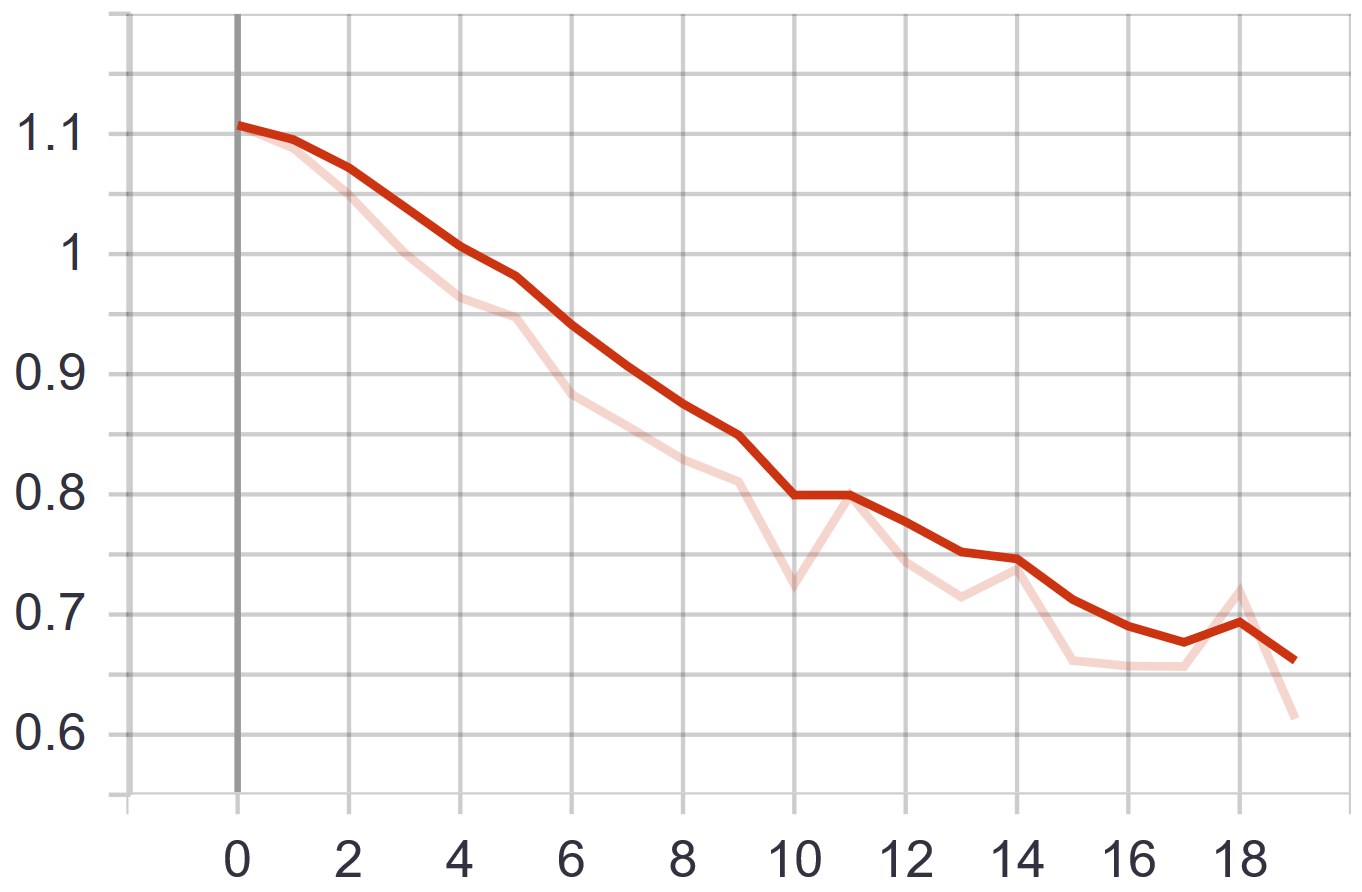
\includegraphics[width=\textwidth]{images/first_model_data_augmentation_loss.png}
        \caption{Loss}
        \label{fig:first_model_data_augmentation_loss}
    \end{subfigure}
    \caption{In comparison to figure~\ref{fig:first_model_graphs} the accuracy and loss are increasing at slower pace. More epochs may improve the results do not seem to be converging after 20 epochs.}
    \label{fig:first_model_data_augmentation_graphs}
\end{figure}

So it is obvious that accuracy on the training data actually decreased.
This is not surprising, since no data is given twice to the model anymore, so no memorization is happening, but as the test accuracy did not change it seems that the desired effect eventuated.
The model accuracy on the training set also seems to be increasing at a lower rate, so more epochs or bigger batches may resolve that problem.

Please note that the training set virtually grew by a factor of 1440 (360 degree + rotations in two axis), therefore enabling the possibility to feed way more data into the model during training without having to expect too much overfitting.

The goal to decrease overfitting seems to be resolved; the difference between training accuracy and test accuracy is negligible small\footnote{Link to respective notebook: \url{https://srp.klawr.de/\#7}}.

\subsection{Feature reduction}
% TODO curse of dimensionality should reduce accuracy... this is not fixed here
Another thing which may be improving model performance is to reduce the size of the input.
The phenomenon known as \textit{curse of dimensionality} describes the possibility of distinct configuration possible as the number of variables is increasing and comes from Richard Bellman initially regarding problems in dynamic programming \cite[p.ix]{Bellman1957}.

The data is already heavily reduced by submitting the data as images with width and height of 32, even though the data is generated as 512 by 512 images. This is because of manual tuning when the data is reasonably small but all features are still recognizable.


The data is initially given in grayscale, because the intended usage allows the images to be converted to grayscale even if the original image has color, because it should not affect the prediction of the symbol.
Albeit being only in grayscales the input is given as an image with three colors (hence the input size \code{[32, 32, 3]}).
One way to reduce the input size is to project the data into one dimension, as suggested by Géron \cite[p.215]{Geron2019}.
Therefore calling the \code{flow\_from\_directory} with another parameter \code{color\_mode='grayscale'} projects the 3-dimensional \code{color\_mode='rgb'} (which is set as default) onto one dimension, changing virtually nothing (the input size is consequently adjusted to \code{[32, 32, 1]}).

The model is subsequently summarized as:
\begin{lstlisting}
Model: "sequential"
_________________________________________________________________
Layer (type)                 Output Shape              Param #   
=================================================================
flatten (Flatten)            (None, 1024)              0         
_________________________________________________________________
dense (Dense)                (None, 32)                32800     
_________________________________________________________________
dense_1 (Dense)              (None, 32)                1056      
_________________________________________________________________
dense_2 (Dense)              (None, 3)                 99        
=================================================================
Total params: 33,955
Trainable params: 33,955
Non-trainable params: 0
_________________________________________________________________
\end{lstlisting}

This is dividing the number of trainable parameters almost by a factor of three and therefore reducing the size of the model from 807kb (from the previous models with 99491 params) to 295kb without losing any measurable performance\footnote{Link to respective notebook: \url{https://srp.klawr.de/\#8}}.

\subsection{Optimizers}

Hitherto the only optimizer looked at is stochastic gradient descent.
Stochastic gradient descent has multiple parameters which can be tweaked, e.g. the learning rate, momentum and whether nesterov is used or not.

Attempts have been made to automate the search for these hyper-parameters.
In this project some alternative optimizers are examined, but not explained into too much detail.
For further explanation please refer to the citations.

In stochastic gradient descent the learning rate is the same for all parameters.
To adjust it for every parameter or even for individual dimensions of the layers may be helpful, but this would need an unproportional increase of cost.

\name{AdaGrad} \cite{Duchi2010} is changing the learning rate for each parameter.
This is done by adjusting the learning rate (starting with a uniform value) on each individual parameter using the magnitude of the gradient for the respective parameter.
While this approach is performing well on some problems it is not useful for other problems.
Nonetheless it serves as baseline for many other optimizers which were developed thereafter, three of which were tested in the tuning algorithm used in this project.

 \name{AdaDelta} \cite{Zeiler2012} is a modified algorithm based on \name{AdaGrad}, which tries to solve AdaGrad's notion to reduce the learning rate constantly by dividing the learning rate again by a exponential decaying average of the gradients.
 This results in a much more stable optimizer which promises to work well in practice.

 \name{RMSProp} \cite{Hinton2012} works similar to \name{AdaDelta} with slightly different update rule.
It is considered to be "generally a good enough choice, whatever your problem" \cite[p.77]{Chollet2017}.

Adam \cite{Kingma2014}\cite{Reddi2018} is the last optimizer included in this project, which is another method of applying an adaptive learning rate for each parameter.
Adam incorporates the previously mentioned idea of momentum into an algorithm similar of RMSProp.

There are other optimizers worth mentioning (namely AdaMax or Nadam) and they may be subject of further investigation.

Worth noticing is that adaptive methods explained here may not work on every model, so it is always worth to use gradient descent with nesterov\cite[p.358]{Geron2019}.

\subsection{Convolutional layers}

Convolutional layers are widely used for image recognition and it therefore is a sensible notion to implement them into the model.
They were introduced by Yann LeCun in a 1998 paper \cite{LeCun1998} to detect handwritten digits.

In this project only two dimensional convolutional layers are used, because the input is two dimensional (after the images are transferred to grayscale).
The difference of convolutional layers to the previously described dense layers is that the parameters trained are not representing the connections of all the nodes of the previous layer to a next one, but a kernel which slides over the input layer and acts as a filter constructing the output layer.
This also means, that the input layer does not have to be flattened before fed into the model.

When training a convolutional layer the parameters trained are the filters which have a predetermined shape.
A two dimensional convolutional layer with eight filters, an input depth of one  and a kernel size of four by four (and one for the bias) has 136 (8 x (1 x 4 x 4 + 1)) parameters to train which is significantly less than previous approaches and does not rely on the size of the input layer, thus making it possible to detect patterns in arbitrarily large images without the necessity of making the model bigger.

The respective equation for a single activation is therefore given by \cite[p. 453]{Geron2019}:
\begin{equation}
z_{i,j,k} = b_k + \sum_{u=1}^{h} \sum_{v=1}^{w} \sum_{k'=1}^{n'} x_{i', j', k'} \times w_{u, v, k', k} 
\end{equation}

Whereas $z$ is the activation value with indices $i$ and $j$ being the position of the node in the output layer and $k$ is representing the index of the filter.
The sum of all input nodes is given by taking the sum of the nodes in the respective directions, which is given by iterating over three axes using the height ($h$), width ($w$) and filter size ($n'$) of the previous layer.
For each of these combinations the respective connection weight $w_{u, v, k', k}$ is multiplied by the input $x_{i', j', k'}$ at the respective position in the previous layer, whereas $i' = i \times s_h + u$ and $j' = j \times s_w$ respectively, with $s_h$ and $s_w$ being the strides\footnote{Strides being the steps taken in each direction for every step. Strides thereby reduce the size of the subsequent layer}.
Additionally each filter has its own bias $b_k$, which is added to the activation.

\begin{figure}
    \centering
    \caption{ The bottom layer is the input represented by a two dimensional layer sized five by five (filter size is one), which has a padding of one (drawn in grey) to ensure the size stays the same using a kernel of size three by three (emphasized by the red, green and blue rectangles.). The stride used is one, meaning the receptive field propagates one input node at each step. Here the process begins at the red rectangle, blue is the second step and green the last (25  steps in total). }
    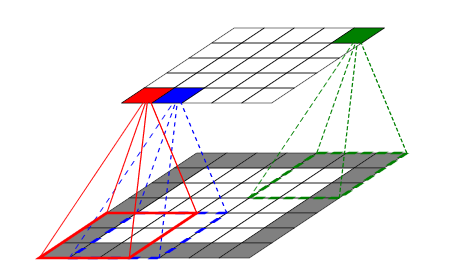
\includegraphics[width=0.6\textwidth]{images/conv_layer.png}
    \label{fig:conv_layer}
\end{figure}

In order for the output to have the same size as the input, numbers have to be added to the input, because a kernel greater than one in any direction can not cross an edge for the input (and the stride has to be 1 by 1).
Therefore padding is used to solve this issue usually by adding zeros around the input, resulting in a technique called zero-padding.

By using convolutional instead of dense layers the model size is again reduced (295kb to 232kb) and the accuracy is increased by a few percentages. By adding pooling the size is again decreased to 149kb and the metrics improve further\footnote{Link to respective notebooks: \url{https://srp.klawr.de/\#9} and \url{https://srp.klawr.de/\#10}}.
Pooling is a technique by which a kernel (similar to the kernel of convolutional layers) scan over the input layer.
In the linked notebook a two by two kernel was used, which takes the max value of the kernel and only forwards the max value, thereby halving the output size in width and height.
Fittingly this is called \name{MaxPooling}.

\subsection{Tuning algorithms}

Attributing to all the possibilities to optimize the model before training some approaches were developed to tune the hyper-parameters automatically.
One way to adjust hyper-parameters is to test each with various values alongside all other hyper parameters being fixed.
This procedure ensures that the optimal set of hyper parameters is used, but may take an inacceptable amount of time, since the number of models created is exponentially growing to the number of hyper parameters which are do be adjusted.
For two hyper parameters this would be equivalent to checking every value on a two dimensional grid, hence the method is called grid search\footnote{If only one hyper parameter is adjusted the procedure is called linear search.}.

Another approach often used in practice is random search.
Random search goes by the notion to randomly assign hyper-parameters and thus testing different models without giving any combination an advantage.
Obviously this does (most likely) not result in optimal result, but in practice this approach is often used, because it does typically provide an acceptable result by checking a broad spectrum of possible configurations.
A notebook was created to show the implementation of \name{keras tuner} in this project at \url{https://srp.klawr.de/\#12}

Some more sophisticated methods are based on the random search approach by repeatedly examining the results of random search and then tuning the hyperparameters favoring those which promise to result in better models.
This approach is called zooming, since one can picture to zoom into the right area of hyperparameters after every iteration.
% TODO check this chapter...
Other approaches try to automate this process entirely.
Popular algorithms are based on Bayesian optimization, but these are not covered in this project and are therefore omitted.

The tuner used in this project is called \name{hyperband} \cite{Li2018}, which is implemented by the library \name{keras-tuner} \cite{Google2019a}.
In essence \name{hyperband} trains models using random search, but limits training for a broad spectrum of hyper-parameters for a few epochs.
By checking which models perform best and keep the most promising ones.
This method promises to be a much better usage of resources and will most likely show the best hyperparameters to choose from.

The final model tuner is designed to accept a \code{Hyperparameters} object which is fed to a function returning the respective model:

% TODO python
\begin{lstlisting}
def create_model(hp):
    model = models.Sequential()
    model.add(layers.Conv2D(2**hp.Int('2**num_filter_0', 4, 6),
        (4,4) ,activation='relu', input_shape=(32, 32, 1)))

    for i in range(hp.Int('num_cnn_layers', 0, 3)):
        filter = 2**hp.Int('2**num_filter_' + str(i), 4, 7)
        model.add(
            layers.Conv2D(filter, (4,4), activation='relu',padding='same'))
        if hp.Boolean('pooling_' + str(i)):
            model.add(layers.MaxPooling2D(2, 2))

    model.add(layers.Flatten())
    for i in range(hp.Int('num_dense_layers', 1, 3)):
        nodes = 2**hp.Int('2**num_nodes_' + str(i), 4, 7)
        model.add(layers.Dense(nodes, activation='relu'))
    
    model.add(layers.Dense(3, 'softmax'))

    optimizers = {
        'adam': Adam(),
        'sgd': SGD(lr=hp.Choice(
            'learning_rate', [0.001, 0.003, 0.007, 0.01 0.03]),
            momentum=hp.Float('momentum', 0.6, 1, 0.1),
            nesterov=hp.Boolean('nesterov')),
        'rms': RMSprop(lr=hp.Choice(
            'learning_rate', [0.001, 0.003, 0.007,0.01, 0.03]))
    }

    model.compile(
        loss='sparse_categorical_crossentropy',
        optimizer=optimizers[hp.Choice('optimizer', list(optimizers.keys())],
        metrics=['acc'])

    return model
\end{lstlisting}

This function enhances \ref{lst:first_model} by implementing hyper-parameters using the \code{Hyperparameters} from \name{keras tuner}.
This is later implemented using the a custom class\footnote{The results were logged using the \name{TensorBoard} API, which is not yet implemented by \name{keras tuner} itself just yet, therefore the tuner is inherited from a custom class}:

\begin{lstlisting}
tuner = customTuner(
    create_model,
    hyperparameters=hp,
    objective='acc',
    max_trials=100,
    executions_per_trial=1,
    directory=log_dir,
    project_name=timestamp)
\end{lstlisting}

The training which was further done by the \code{fit} function is now done by the tuner's \code{search} function:

\begin{lstlisting}
tuner.search(
    train_dataset,
    validation_data=validation_dataset,
    epochs=30,
    steps_per_epoch=100,
    validation_steps=100,
    verbose=0,
    callbacks=callbacks)
\end{lstlisting}

Another note to take here is that the generators used in \ref{ch:data_augmentation} were replaced by manual augmenting the data and later preprocessing them using protocol buffers(\name{protobufs})\footnote{For this several advances have been made. The final notebook using those can be reviewed at \url{https://srp.klawr.de/\#11}}.
By preprocessing the image data beforehand significantly reduces training time.
The code used for this can be reviewed here: \url{https://srp.klawr.de/\#13}.

After reviewing the data the data increased accuracy to 96,7\% on the test data with a model size of 4,3mb.

\subsection{Increasing the training set}

After a lot of time tuning the model and trying to enhance the tuner, the raw training data was more than tripled (to 1000 examples for each symbol in the training data) and then augmented using 32 repetitions resulting in a dataset of 96000 (almost) distinct images.

Using this dataset an accuracy of of over 99\% got reached on nearly any test. This is making minimizing the model the next goal.
The final model has a size of 207kb with 99,3\% accuracy and a loss of 0.04, which are satisfactory results.

The model is defined as:
\begin{lstlisting}
model = models.Sequential()
model.add(layers.Conv2D(16, (4,4), activation='relu', padding='same',input_shape=(32, 32, 1)))
model.add(layers.MaxPooling2D(2,2))
model.add(layers.Conv2D(32, (4,4), activation='relu', padding='same'))
model.add(layers.MaxPooling2D(2,2))
model.add(layers.Flatten())
model.add(layers.Dense(3, 'softmax'))

optimizer = Adam()
model.compile(loss='sparse_categorical_crossentropy', optimizer=optimizer,metrics=['acc'])
\end{lstlisting}

The final code for the model creation can be reviewed at \url{srp.klawr.de/\#14}.